\documentclass[10pt]{article}
\usepackage{icmlko}

\icmlmeta{IP 파운데이션 월드모델}{473}{배급사가 가리고 있던 것}{영화 국적이 씨앗 셋에서 재현됐고, 분해가 네 가설을 한꺼번에 죽였다 --- 그리고 배급사 축을 끄자 그 열이 3.5배로 커졌다}

\begin{document}

\twocolumn[
\icmlheader

\begin{abstract}
직전 사이클은 규칙이 밀어낸 2순위 열(영화 \texttt{국적})이 그 도메인
$2\sigma$의 5배로 살아나는 것을 보고도 사전등록 부칙 때문에 판정하지
못했다. 이번엔 그 열을 1순위로 다시 등록하고 씨앗 셋으로 재현하며 팔
일곱으로 분해했다. \textbf{재현했다} --- 신호 몫 $+0.0577$, 씨앗
셋이 각각 $+0.0579 \cdot +0.0555 \cdot +0.0597$로 전부 $2\sigma$(0.0137)
위, 위약 6/6, 판 $+0.0063$. 자도 고쳤다: 분모를 은퇴한 3,369에서
837 정본 3,775로 옮겼고, \textbf{영화 도메인 씨앗 SD를 처음 쟀다}
(0.0027 --- 유보 406행짜리 얇은 도메인인데 예상보다 한 자릿수 작다).

분해가 네 가설을 한꺼번에 죽였다. \textbf{전이 누출은 신호를 부풀린
게 아니라 눌렀다} --- 집단 크기를 학습 구간만으로 세면 범주가
다섯에서 셋으로 줄어드는데 점수는 오히려 $+0.0168$ 올라간다. 순서
인코딩도 아니다(원핫이 순서형과 같다 --- \emph{범주 정체성}이 낸다).
파싱 쓰레기 21행 정정은 소수 넷째 자리까지 무변. 그리고 마지막
팔이 그림을 바꿨다: \textbf{배급사 축을 끄면} 영화가 0.4835에서
0.1349로 무너지고 국적을 넣으면 0.3397로 돌아온다 --- 이득
$+0.2048$, 배급사가 있을 때의 \textbf{3.5배}. 국적은 배급사가 나르던
정보를 크게 대신할 수 있고, 배급사가 있어도 고유분 $+0.0577$을 더
준다.
\end{abstract}
]

\section{재현과 자}

884는 씨앗 하나로 쟀고 자의 분모가 은퇴한 숫자(11도메인 시대 유보
3,369)였다. 이번에 둘 다 고쳤다. 영화 씨앗 SD 0.0027은 이 실험실이
얇은 도메인에서 잰 값(0.016$\sim$0.024)보다 훨씬 작다 --- 그래서
실질 문턱을 정한 것은 씨앗 분산이 아니라 \textbf{위약 분산}
($2\times$뽑기SD $= 0.0285$)이었고, 신호는 그것도 두 배로 넘었다.

세 기준선을 다 적는다: 없이 0.4835, 값셔플 0.4849(판정 분모 ---
사전 고정), 행셔플 0.4750. 어느 분모로 재도 $2\sigma$의
4.3$\sim$4.9배다.

\begin{figure}[t]
\centering
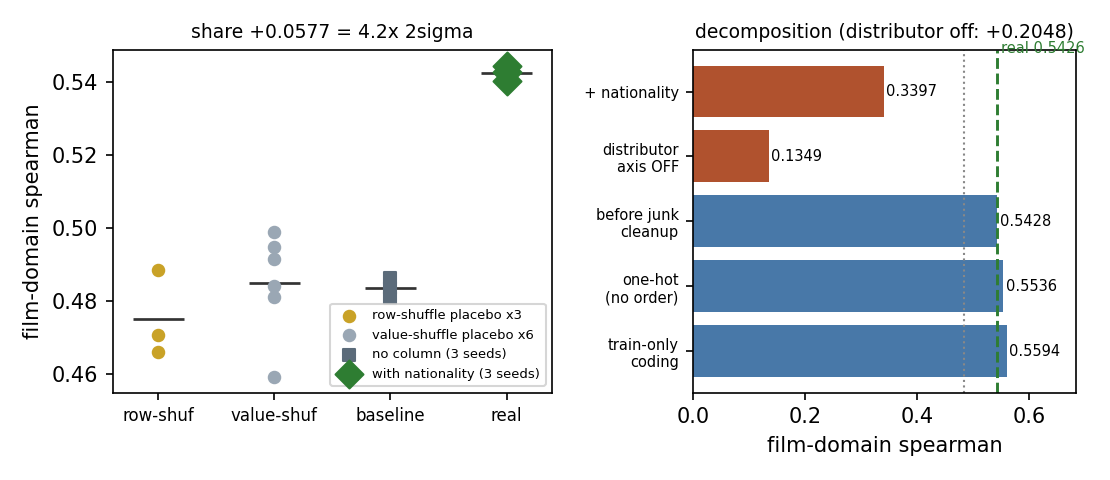
\includegraphics[width=\linewidth]{figs/hidden.png}
\caption{왼쪽: 네 팔. 진짜(초록 마름모 셋)가 위약 구름에서 완전히
떨어져 있고 씨앗 간 흩어짐이 위약 흩어짐보다 훨씬 작다. 오른쪽:
분해. 학습-구간-전용 코딩이 진짜보다 \emph{위}에 있고, 배급사 축을
끈 쌍(주황)이 그 열의 크기를 드러낸다. 전부 산출물에서 계산했다.}
\end{figure}

\section{배급사를 끄면 보이는 것}

판 밖 대리 모형에서는 이 관계가 억제변수로 읽혔다(배급사를 통제하면
국적의 부분상관이 오히려 커진다). 판 하네스 안에서는 다른 얼굴이
보인다 --- 배급사는 영화 도메인의 기둥이고(끄면 0.4835$\to$0.1349),
국적은 그 기둥이 없을 때 절반 이상을 혼자 떠받친다. 둘 다 참일 수
있다: 겹침이 크고, 그 위에 고유분이 남는다. 실무적으로 중요한 것은
\textbf{정상 판(배급사가 있는 상태)에서 국적이 $2\sigma$의 4.2배를
더 준다}는 쪽이다.

\section{그래도 채택하지 않는다 --- 그리고 그 대신 한 일}

규약 12는 집 밖 짝 둘을 요구하는데 \textbf{영화에는 집 밖 짝이
없다}. 같은 종류의 열을 다른 도메인에서 재현하는 길도 실측으로
죽었다(세계애니 원산지는 98.7\%가 일본, 만화는 판 안에서 상수,
게임엔 열이 없다). 그래서 다른 문을 열었다: 9월 말 수확을 기다리는
\textbf{봉인 30편에 국적 팔을 오늘 얼렸다}(첫 봉인작 개봉 이틀
전 --- 라벨이 생기기 전). 채점 규칙도 지금 못박았다. 국적 팔이 대조
팔보다 높고 그 차가 대조 밴드 밖이면 전향에서도 사는 것이고,
\emph{더 낮으면} 이번 집안 통과를 판 안 과적합으로 재분류한다.

\section{교훈}

\textbf{분해는 방어가 아니라 발견이다.} 네 팔은 누출을 방어하려고
붙였는데, 그중 둘이 신호에 대해 새로운 것을 알려줬다 --- 전이가
신호를 누르고 있었다는 것, 그리고 국적이 배급사의 상당 부분을
대신한다는 것. 방어용으로 설계한 팔에서 가장 많이 배웠다.

\end{document}
